\chapter{时间相干与一阶（振幅）干涉}
\label{chap:e09}

\begin{chapteropening}
到这里，我们已经知道光是一组模式的激发，其正频率场算符 \(\hat E^{(+)}\) 是第 \ref{chap:e05} 章引入的；而探测器只数强度、看不见电场的相位这件事，正是第 \ref{chap:e07} 章光电探测所讲的（一个光学周期只有几飞秒，任何探测器都太"慢"，只能把振荡抹平留下能量）。我们也知道一束光"记得自己相位"的时间只有相干时间 \(\tau_c\simeq1/\Delta\nu\) 那么长（第 \ref{chap:e02} 章）。可是既然相位看不见，我们凭什么谈论"相干"？答案是干涉：把一束光劈成两路、走不同的光程再合到一起，相位差就会在\emph{强度}上显形——亮纹、暗纹，一道一道的条纹。本章要做的，是把抽象的一阶相干度 \(g^{(1)}(\tau)\) 落到一台看得见摸得着的干涉仪上：推出条纹强度公式，定义条纹可见度（visibility），证明"可见度就是电场还记得多少相位"的直接读数；再顺着维纳--辛钦定理（Wiener--Khinchin theorem）搭一座桥，说明为什么"条纹随光程差变淡的快慢"竟能反过来告诉我们谱线的形状——这正是傅里叶变换光谱学的原理。最后我们把这套"时间延迟版"的相干推广到"两点空间版"，交到下一章 van Cittert--Zernike 定理与强度干涉的手上。
\end{chapteropening}

\section{从一条光路到两条光路}
\label{sec:e09-two-beams}

先把干涉仪画出来。最干净的例子是迈克尔逊干涉仪（Michelson interferometer）：一束光打到分束镜上，一半射向固定镜、一半射向可移动镜，两路各自原路返回、在分束镜后重新合并，一起落到同一个探测器上。两条光路的长度一般不等，差一个光程 \(\Delta\)（单位 cm）。杨氏双缝（Young's double slit）在几何上是它的兄弟：同一束光穿过两条缝，到达屏上某点时也走了不等的两段路，只不过那里的路程差来自\emph{空间}的两个取样点，本章末尾我们会回到这一点。现在先盯住迈克尔逊这种"同一束光、两段光程"的时间版本。

探测器面上的场，是两路场的叠加：
\[
  \hat E_{\rm det}(t)=\hat E_1(t)+\hat E_2(t),
\]
其中 \(\hat E_1\)、\(\hat E_2\) 是两路各自到达探测器的正频率场算符（第 \ref{chap:e05} 章）。探测器"太慢"，逐个光学周期的振荡它抹平了，留下的是在响应时间里平均的强度，正比于场模平方。于是这一点的平均强度是
\[
  I=\big\langle \hat E_{\rm det}^{(-)}(t)\,\hat E_{\rm det}^{(+)}(t)\big\rangle
   =\big\langle |\hat E_1+\hat E_2|^2\big\rangle .
\]
把模平方展开。这是最普通的代数 \(|a+b|^2=|a|^2+|b|^2+a^\ast b+ab^\ast\)，逐项取平均：
\[
  I=\underbrace{\big\langle|\hat E_1|^2\big\rangle}_{I_1}
   +\underbrace{\big\langle|\hat E_2|^2\big\rangle}_{I_2}
   +\big\langle \hat E_1^\ast \hat E_2\big\rangle
   +\big\langle \hat E_1 \hat E_2^\ast\big\rangle .
\]
前两项 \(I_1,I_2\) 是两路各自单独打开时的强度（若挡住另一路就只剩它）。后两项互为复共轭，两个复共轭相加等于二倍实部，所以
\begin{equation}
  I=I_1+I_2+2\,\mathrm{Re}\big\langle \hat E_1^\ast(t)\,\hat E_2(t)\big\rangle .
  \label{eq:e09-interference-raw}
\end{equation}
\begin{formulaexplain}
\(I_1,I_2\) 是两路各自的强度；最后那个交叉项 \(\langle\hat E_1^\ast\hat E_2\rangle\) 是"两路场彼此还记得多少"的相关。干涉的一切，全藏在这一项里。
\end{formulaexplain}

逐项交代。\(I_1,I_2\) 有强度量纲（CGS 下 \({\rm erg\,s^{-1}\,cm^{-2}}\) 量级，这里只用它们的相对大小）。真正携带信息的是交叉项 \(\langle\hat E_1^\ast(t)\hat E_2(t)\rangle\)：如果两路场毫无关系，这个平均等于零，探测器上就只有平淡的 \(I_1+I_2\)，没有条纹；如果两路场高度相关，交叉项很大，随光程差一扫就出现明暗对比强烈的条纹。所以\textbf{条纹的深浅，直接量的就是这条交叉相关}。

现在要把交叉项算清楚。关键的物理事实是：第 2 路只是第 1 路那束光被延迟、被搬动了一个光程 \(\Delta\) 而已——它们来自同一个源场，只是取自不同时刻。把归一化的复场记作 \(\varepsilon(t)\)（满足 \(\langle|\varepsilon|^2\rangle=1\)），两路可写成
\[
  \hat E_1(t)=\sqrt{I_1}\,\varepsilon(t),\qquad
  \hat E_2(t)=\sqrt{I_2}\,\varepsilon(t-\tau),\qquad
  \tau=\frac{\Delta}{c}.
\]
这里 \(\tau=\Delta/c\) 是光程差换算成的\emph{时间延迟}（单位 s），\(c\) 是光速。第 2 路的场，就是第 1 路的场倒退 \(\tau\) 时间取到的值。于是交叉项变成同一个场在相隔 \(\tau\) 的两个时刻的相关：
\[
  \big\langle \hat E_1^\ast(t)\,\hat E_2(t)\big\rangle
  =\sqrt{I_1 I_2}\,\big\langle \varepsilon^\ast(t)\,\varepsilon(t-\tau)\big\rangle .
\]
这里出现的是 \(\varepsilon(t-\tau)\)（第 2 路延迟了 \(\tau\)），而下面 \(g^{(1)}\) 的标准定义里写的是 \(\varepsilon(t+\tau)\)——两者相差一个复共轭，别急着划等号。用平稳性（相关只依赖延迟、不依赖绝对时刻）把时间原点平移 \(t\to t+\tau\)：
\[
  \big\langle \varepsilon^\ast(t)\,\varepsilon(t-\tau)\big\rangle
  =\big\langle \varepsilon^\ast(t+\tau)\,\varepsilon(t)\big\rangle
  =\big[g^{(1)}(\tau)\big]^\ast=g^{(1)}(-\tau) .
\]
好在最终代进式 \eqref{eq:e09-interference-raw} 的只是这一项的\emph{实部}、并会用到它的\emph{模}；而 \(|g^{(1)}|\) 是偶函数、实部对取复共轭又不变，所以把它直接换写成 \(g^{(1)}(\tau)\) 对条纹的模与实部\emph{毫无影响}。据此，它正是第 \ref{chap:e08} 章定义过的一阶相干度（first-order/amplitude coherence）。把归一化的一阶时间相干度记作
\begin{equation}
  g^{(1)}(\tau)=
  \frac{\big\langle \varepsilon^\ast(t)\,\varepsilon(t+\tau)\big\rangle}
       {\big\langle |\varepsilon(t)|^2\big\rangle},
  \qquad g^{(1)}(0)=1 ,
  \label{eq:e09-g1-def}
\end{equation}
\begin{formulaexplain}
\(g^{(1)}(\tau)\) 是同一束光相隔 \(\tau\) 的电场相关，除以自身强度归一化。它是复数：模 \(|g^{(1)}|\) 说"还记得多少"，幅角说"相位差了多少"。\(\tau=0\) 时场和自己完全相关，\(g^{(1)}(0)=1\)。
\end{formulaexplain}
其中 \(\tau\) 是时间延迟（单位 s），\(g^{(1)}\) 无量纲。它是复数：\(|g^{(1)}(\tau)|\) 从 1（\(\tau=0\)，完全相干）随延迟增大衰减到 0（相位记忆完全丢失）；它的幅角记录相位差。对平稳（stationary）光场，这个相关只依赖延迟 \(\tau\)，不依赖绝对时刻 \(t\)——这一点后面反复要用。

把交叉项代回式 \eqref{eq:e09-interference-raw}。这里要做一件对物理很关键的拆分。相干度 \(g^{(1)}(\tau)\) 的相位里其实混着两种快慢完全不同的东西：一种是载波相位（carrier phase），来自光程差在中心频率 \(\bar\nu\) 上累积的振荡；另一种是缓慢变化的残余相位。因为光程差每变化一个波长 \(\lambda\)，载波相位就转过整整 \(2\pi\)，而 \(|g^{(1)}|\) 几乎纹丝不动，所以把载波单独乘出来最自然。先定义载波相位
\[
  \delta=\frac{2\pi\Delta}{\lambda}=2\pi\bar\nu\,\tau ,
\]
再把这个载波从 \(g^{(1)}\) 里\emph{除掉}，得到一个只剩缓慢变化的复量，记作 \(\tilde g(\tau)\)（注意它是一个\emph{新符号}，不是 \(\arg g^{(1)}\) 本身）：
\[
  \tilde g(\tau)\equiv e^{+i2\pi\bar\nu\tau}\,g^{(1)}(\tau)
  =\big|g^{(1)}(\tau)\big|\,e^{\,i\varphi(\tau)} .
\]
乘上一个模为 1 的相位因子不改变模，所以 \(|\tilde g|=|g^{(1)}|\)；这里 \(\varphi(\tau)\) 就是\emph{去掉载波后剩下的缓慢残余相位}（无量纲，单位 rad），谱线对称时 \(\varphi\equiv0\)。把这条定义反解出 \(g^{(1)}\)：
\[
  g^{(1)}(\tau)=e^{-i2\pi\bar\nu\tau}\,\tilde g(\tau)
  =\big|g^{(1)}(\tau)\big|\,e^{\,i[\varphi(\tau)-\delta]} .
\]
于是取实部（\(\cos\) 是偶函数，\(\cos(\varphi-\delta)=\cos(\delta-\varphi)\)）得 \(\mathrm{Re}\,g^{(1)}=|g^{(1)}|\cos\!\big(\delta-\varphi(\tau)\big)\)，代回式 \eqref{eq:e09-interference-raw} 得到本节的中心结果——双光束干涉的条纹公式：
\begin{equation}
  I(\delta)=I_1+I_2+2\sqrt{I_1 I_2}\;\big|g^{(1)}(\tau)\big|\,
  \cos\!\big(\delta-\varphi(\tau)\big),
  \qquad \delta=\frac{2\pi\Delta}{\lambda},\ \ \tau=\frac{\Delta}{c}.
  \label{eq:e09-fringe}
\end{equation}
\begin{formulaexplain}
条纹强度 = 两路本底 \(I_1+I_2\) + 一个随光程差起伏的余弦项。余弦让明暗交替，它的\emph{振幅}正比于 \(|g^{(1)}(\tau)|\)——电场记得越多，条纹起伏越大。载波相位 \(\delta=2\pi\Delta/\lambda\) 是我们移动镜子扫的旋钮；\(\varphi(\tau)\) 是去掉载波后的缓慢残余相位，谱线对称时为零。
\end{formulaexplain}

把这条式子读透。\(\delta=2\pi\Delta/\lambda\) 是移动镜子直接控制的相位：镜子平移半个波长（光程差变一个波长），\(\delta\) 转过 \(2\pi\)，条纹走过明暗各一遍。所以随着我们扫描 \(\Delta\)，探测器读数在 \(I_{\max}\) 和 \(I_{\min}\) 之间来回摆——这就是条纹。摆动的幅度是 \(2\sqrt{I_1 I_2}\,|g^{(1)}(\tau)|\)：它有两个因子，\(2\sqrt{I_1I_2}\) 是两路光强搭配得好不好（等光强时最大），\(|g^{(1)}(\tau)|\) 是电场在延迟 \(\tau\) 后还记得多少相位。若 \(|g^{(1)}|=1\)，条纹在 \(I_1+I_2\) 上下满幅摆动；若 \(|g^{(1)}|=0\)，余弦项消失，探测器上一片均匀，没有条纹。换句话说：\textbf{条纹的存在与深浅，就是一阶相干的直接显影}。下一节我们把"深浅"这件事量化成一个标准数字。

\section{条纹可见度就是相干度的读数}
\label{sec:e09-visibility}

肉眼看条纹，第一印象是"清不清楚"——亮纹和暗纹反差大就清楚，反差小就模糊。把这个印象变成可测量的数字，就是条纹可见度（fringe visibility），由 Michelson 最早引入：
\begin{equation}
  \mathcal V=\frac{I_{\max}-I_{\min}}{I_{\max}+I_{\min}} .
  \label{eq:e09-visibility-def}
\end{equation}
\begin{formulaexplain}
\(\mathcal V\) 用最亮纹 \(I_{\max}\) 和最暗纹 \(I_{\min}\) 的反差除以它们的和。全黑到全亮时 \(\mathcal V=1\)，一片灰没有条纹时 \(\mathcal V=0\)。它是"条纹有多清楚"的标准刻度。
\end{formulaexplain}
\(I_{\max}\)、\(I_{\min}\) 分别是扫描 \(\delta\) 时探测器读到的最大、最小强度，\(\mathcal V\) 无量纲，介于 0 和 1 之间。为什么用这个组合而不用别的？因为它\emph{自动约掉总亮度}：把光源调亮一倍，\(I_{\max},I_{\min}\) 同时翻倍，比值不变。可见度只关心"反差"，不关心"多亮"，正好对应我们想问的"相干性"。

现在把式 \eqref{eq:e09-fringe} 代进去算。扫描 \(\delta\) 时，余弦在 \(+1\) 和 \(-1\) 之间取值（残余相位 \(\varphi(\tau)\) 变化很慢，在一条条纹的尺度上可当常数，只是给条纹整体平移一点，不改变峰谷高度）：
\[
  I_{\max}=I_1+I_2+2\sqrt{I_1 I_2}\,|g^{(1)}(\tau)|
  \quad(\cos=+1),
\]
\[
  I_{\min}=I_1+I_2-2\sqrt{I_1 I_2}\,|g^{(1)}(\tau)|
  \quad(\cos=-1).
\]
两式相减，本底 \(I_1+I_2\) 抵消，余下两倍的余弦振幅：
\[
  I_{\max}-I_{\min}=4\sqrt{I_1 I_2}\,|g^{(1)}(\tau)| .
\]
两式相加，余弦振幅抵消，余下两倍本底：
\[
  I_{\max}+I_{\min}=2\,(I_1+I_2).
\]
相除，那个公共的 2 约掉，得到可见度与相干度的桥梁：
\begin{equation}
  \mathcal V(\tau)=\frac{2\sqrt{I_1 I_2}}{I_1+I_2}\,\big|g^{(1)}(\tau)\big| .
  \label{eq:e09-visibility-g1}
\end{equation}
\begin{formulaexplain}
可见度 = 光强搭配因子 \(2\sqrt{I_1I_2}/(I_1+I_2)\) 乘以相干度模 \(|g^{(1)}(\tau)|\)。前者只和两路亮度比有关，后者才是光本身的相干性。等光强时前者为 1，可见度\emph{就是} \(|g^{(1)}|\)。
\end{formulaexplain}

这条式子把两件事干净地分开了。第一个因子 \(2\sqrt{I_1 I_2}/(I_1+I_2)\) 纯粹是几何搭配：它是两路光强的几何平均比算术平均，永远 \(\le 1\)，只有当 \(I_1=I_2\) 时才等于 1（这是均值不等式，几何平均等于算术平均当且仅当两数相等）。它衡量的是"仪器有没有把两路调成等亮"，和光的相干性无关。第二个因子 \(|g^{(1)}(\tau)|\) 才是物理主角。于是在实验里人们总是刻意把两路调成等光强 \(I_1=I_2\)，此时搭配因子为 1，可见度和相干度直接相等：
\begin{equation}
  \boxed{\;\mathcal V(\tau)=\big|g^{(1)}(\tau)\big|\quad(I_1=I_2)\;}
  \label{eq:e09-visibility-equals-g1}
\end{equation}
\begin{formulaexplain}
等光强时，你在干涉图上量到的条纹清晰度 \(\mathcal V\)，\emph{就是}那个抽象的一阶相干度的模 \(|g^{(1)}(\tau)|\)。抽象的"电场还记得相位"变成了看得见的条纹对比度。
\end{formulaexplain}

这就是本章想让你记住的第一句话：\textbf{条纹可见度是"电场还记得相位"的直接读数}。第 \ref{chap:e08} 章里 \(g^{(1)}\) 是一个写在算符平均里的抽象对象，你没法直接"看到"它；现在它有了肉眼可读的化身——把干涉仪的延迟调到 \(\tau\)，数一数亮纹暗纹的反差，得到的就是 \(|g^{(1)}(\tau)|\)。相位那件探测器"看不见"的东西，通过干涉在强度上留下了它的影子，而可见度就是这道影子的深浅。

顺带一提，等光强双缝的两种极端很好记：\(\mathcal V=1\) 表示完全相干，条纹从全黑到全亮，天文上对应"这条基线还完全没分辨开源"；\(\mathcal V=0\) 表示完全不相干，屏上只有两缝各自照明的平坦叠加，没有条纹，对应"源在这个尺度上已被彻底分辨、相干性洗光"。真实观测几乎都落在两者之间，可见度是个介于 0 和 1 的小数，它的具体数值携带着我们想要的信息。

\section{相干长度与相干时间}
\label{sec:e09-coherence-length}

式 \eqref{eq:e09-visibility-equals-g1} 说可见度随延迟 \(\tau\) 变化。那它怎么变？物理直觉很清楚：延迟越大，第 2 路取自越久以前的场，而光"记得自己相位"的时间只有相干时间 \(\tau_c\simeq1/\Delta\nu\)（第 \ref{chap:e02} 章）那么长；一旦延迟超过 \(\tau_c\)，两路的相位早已各走各的、失去关联，\(|g^{(1)}|\to0\)，条纹随之消失。所以：

\begin{quote}
\textbf{条纹随光程差增大而变淡，衰减的特征尺度就是相干长度。}
\end{quote}

把相干时间换算成光走过的距离，就是相干长度（coherence length）：
\begin{equation}
  \ell_c=c\,\tau_c\simeq\frac{c}{\Delta\nu}\simeq\frac{\lambda^2}{\Delta\lambda},
  \qquad
  \Delta\nu\simeq\frac{c\,\Delta\lambda}{\lambda^2}.
  \label{eq:e09-coherence-length}
\end{equation}
\begin{formulaexplain}
\(\ell_c\) 是"两路光程差还能看到条纹"的最大尺度（单位 cm）。它等于相干时间 \(\tau_c\) 乘光速。带宽 \(\Delta\nu\) 越宽（或 \(\Delta\lambda\) 越大），相干长度越短，条纹越早消失。
\end{formulaexplain}
逐项交代。\(\ell_c\) 单位是 cm（或 m）；\(\tau_c\) 是相干时间（s）；\(\Delta\nu\) 是频率带宽（Hz）；\(\lambda\) 是中心波长，\(\Delta\lambda\) 是波长带宽。最后一步的带宽换算 \(\Delta\nu\simeq c\,\Delta\lambda/\lambda^2\) 来自对 \(\nu=c/\lambda\) 求微分（\(|{\rm d}\nu|=(c/\lambda^2)|{\rm d}\lambda|\)），与第 \ref{chap:e02} 章一致。物理含义一句话：\emph{当两路光程差超过 \(\ell_c\)，条纹就基本看不见了}。它是干涉仪"能容忍多大光程失配"的硬指标。

代入真实数字，感受这个尺度跨了多少量级。

\paragraph{白光。}肉眼所见的白光带宽极宽，取 \(\lambda\simeq550\,{\rm nm}\)、\(\Delta\lambda\simeq300\,{\rm nm}\)（整个可见光）：
\[
  \Delta\nu\simeq\frac{(3\times10^{10}\,{\rm cm\,s^{-1}})(3\times10^{-5}\,{\rm cm})}
  {(5.5\times10^{-5}\,{\rm cm})^2}\simeq3\times10^{14}\,{\rm Hz},
  \quad
  \tau_c\simeq3.4\times10^{-15}\,{\rm s},
  \quad
  \ell_c\simeq1\,\mu{\rm m}.
\]
白光的相干长度只有大约一微米——两三个波长！这正是为什么用白光看迈克尔逊干涉时，只有两臂几乎完全等长的一小段范围内能看到彩色条纹，稍微一移就糊掉。它也解释了肥皂膜、油膜上的彩色干涉为什么只在膜很薄时出现。

\paragraph{窄带滤光片。}加一片 \(\Delta\lambda=1\,{\rm nm}\) 的滤光片，中心 \(\lambda=550\,{\rm nm}\)：\(\Delta\nu\simeq1\times10^{12}\,{\rm Hz}\)，\(\tau_c\simeq1\,{\rm ps}\)，\(\ell_c\simeq0.3\,{\rm mm}\)。相干长度一下涨到亚毫米——现在两臂允许差上零点几毫米还看得见条纹。Guerin 等人的恒星聚束实验用的正是这个量级：\(\lambda\simeq780\,{\rm nm}\)、\(\Delta\lambda=1\,{\rm nm}\) 给出 \(\tau_c\simeq2\,{\rm ps}\)、\(\ell_c\simeq0.6\,{\rm mm}\) \citep{2017MNRAS.472.4126G}。

\paragraph{激光。}一台单频激光器带宽可窄到 \(\Delta\nu=1\,{\rm MHz}\)：\(\tau_c=1\,\mu{\rm s}\)，\(\ell_c=c\tau_c=300\,{\rm m}\)。相干长度几百米——这就是为什么激光能做长臂干涉（乃至引力波探测器那样公里级的臂长）而白光绝无可能。把带宽再压到 kHz，相干长度进入几百公里。

一张表把跨越十几个数量级的图景收进眼底：从白光的微米，到窄带的亚毫米，到激光的百米，相干长度完全由带宽决定。记住这条链子，它在后面每一次谈"能容忍多大延迟/光程差"时都会回来。

\section{维纳--辛钦桥：条纹衰减反推谱线}
\label{sec:e09-wiener-khinchin}

前一节说 \(|g^{(1)}(\tau)|\) 随 \(\tau\) 在相干时间尺度上衰减，但没说\emph{按什么形状}衰减——是先慢后快，还是指数下滑，还是振荡着掉下去？这个形状不是随便的，它由光的\textbf{谱线形状}唯一决定。把这层关系讲清楚的，是维纳--辛钦定理：\(g^{(1)}(\tau)\) 与归一化功率谱互为傅里叶变换。这座桥有个惊人的推论——\emph{测条纹随延迟怎么衰减，就能反推出谱线长什么样}，这正是傅里叶变换光谱学（Fourier-transform spectroscopy）的原理。第 \ref{chap:e02} 章预告过它，这里把它自足地建立起来。

推导只需一个物理输入：平稳光场的不同频率分量互不相关。先把复场按频率展开（这是第 \ref{chap:e02} 章的傅里叶分析，只保留正频率部分，对应第 \ref{chap:e05} 章的 \(\hat E^{(+)}\)）：
\[
  \varepsilon(t)=\int_0^\infty \tilde\varepsilon(\nu)\,e^{-i2\pi\nu t}\,{\rm d}\nu,
  \qquad
  \varepsilon^\ast(t)=\int_0^\infty \tilde\varepsilon^\ast(\nu')\,e^{+i2\pi\nu' t}\,{\rm d}\nu' .
\]
其中 \(\tilde\varepsilon(\nu)\) 是频率 \(\nu\) 处的复振幅。把两者相乘、对延迟 \(\tau\) 写出一阶相关 \(G^{(1)}(\tau)=\langle\varepsilon^\ast(t)\varepsilon(t+\tau)\rangle\)：
\[
  G^{(1)}(\tau)
  =\int_0^\infty\!\!\int_0^\infty
  \big\langle \tilde\varepsilon^\ast(\nu')\,\tilde\varepsilon(\nu)\big\rangle\,
  e^{+i2\pi\nu' t}\,e^{-i2\pi\nu(t+\tau)}\,{\rm d}\nu\,{\rm d}\nu' .
\]
现在用上那个唯一的物理输入。光场\emph{平稳}——统计性质不随时间原点改变——数学上强制不同频率分量互不相关，只有同一频率才有非零关联。这是一个标准结果（平稳过程的谱表示定理，可当作已知）：
\[
  \big\langle \tilde\varepsilon^\ast(\nu')\,\tilde\varepsilon(\nu)\big\rangle
  =S(\nu)\,\delta(\nu-\nu') ,
\]
其中 \(S(\nu)\ge0\) 就是功率谱密度（power spectral density，即谱线形状），\(\delta\) 是狄拉克函数。之所以必须这样，是因为若 \(\nu\ne\nu'\) 的关联不为零，上式里就会残留 \(e^{i2\pi(\nu'-\nu)t}\) 这种含 \(t\) 的因子，破坏"结果只依赖 \(\tau\) 不依赖 \(t\)"的平稳性。代入后 \(\delta(\nu-\nu')\) 把一重积分吃掉（令 \(\nu'=\nu\)），含 \(t\) 的指数 \(e^{+i2\pi\nu t}e^{-i2\pi\nu t}=1\) 恰好抵消：
\[
  G^{(1)}(\tau)=\int_0^\infty S(\nu)\,e^{-i2\pi\nu\tau}\,{\rm d}\nu .
\]
最后除以 \(\tau=0\) 时的值 \(G^{(1)}(0)=\int S(\nu)\,{\rm d}\nu\)（总功率）归一化，得到维纳--辛钦定理：
\begin{equation}
  g^{(1)}(\tau)=
  \frac{\displaystyle\int_0^\infty S(\nu)\,e^{-i2\pi\nu\tau}\,{\rm d}\nu}
       {\displaystyle\int_0^\infty S(\nu)\,{\rm d}\nu} .
  \label{eq:e09-wiener-khinchin}
\end{equation}
\begin{formulaexplain}
一阶相干度 \(g^{(1)}(\tau)\) 是归一化功率谱 \(S(\nu)\) 的傅里叶变换。谱线越宽，\(g^{(1)}\) 衰减越快（相干时间越短）；谱线的具体形状，决定条纹包络的具体形状。
\end{formulaexplain}
\(S(\nu)\) 是功率谱密度（谱线形状），\(\nu\) 单位 Hz；分母把总功率归一化，保证 \(g^{(1)}(0)=1\)。这条式子把"时域的相干"和"频域的谱线"锁成一对傅里叶变换。它立刻给出前一节相干时间的来历：谱线越宽（\(\Delta\nu\) 越大），它的傅里叶变换越窄（\(\tau_c\simeq1/\Delta\nu\) 越小），条纹越早消失。下面两个例子把"谱线形状 → 条纹衰减形状"的对应具体算出来，用的都是标准傅里叶变换对。

\paragraph{例一：矩形谱 → sinc 衰减。}设谱线是一段宽度为 \(\Delta\nu\)、中心在 \(\bar\nu\) 的矩形（理想的平顶窄带滤光片），归一化后 \(S(\nu)=1/\Delta\nu\)（在带内），代入式 \eqref{eq:e09-wiener-khinchin}。令 \(\nu=\bar\nu+f\)，\(f\in[-\Delta\nu/2,\,\Delta\nu/2]\)：
\[
  g^{(1)}(\tau)=\frac{1}{\Delta\nu}\int_{-\Delta\nu/2}^{\Delta\nu/2}
  e^{-i2\pi(\bar\nu+f)\tau}\,{\rm d}f
  =\frac{e^{-i2\pi\bar\nu\tau}}{\Delta\nu}
  \int_{-\Delta\nu/2}^{\Delta\nu/2}e^{-i2\pi f\tau}\,{\rm d}f .
\]
里面是最基本的指数积分 \(\int e^{-i2\pi f\tau}{\rm d}f=e^{-i2\pi f\tau}/(-i2\pi\tau)\)，代上下限并用 \(e^{-ix}-e^{+ix}=-2i\sin x\)：
\[
  \int_{-\Delta\nu/2}^{\Delta\nu/2}e^{-i2\pi f\tau}\,{\rm d}f
  =\frac{e^{-i\pi\Delta\nu\tau}-e^{+i\pi\Delta\nu\tau}}{-i2\pi\tau}
  =\frac{-2i\sin(\pi\Delta\nu\tau)}{-i2\pi\tau}
  =\frac{\sin(\pi\Delta\nu\tau)}{\pi\tau} .
\]
除以 \(\Delta\nu\)，凑成标准的 sinc 函数 \({\rm sinc}(x)\equiv\sin(\pi x)/(\pi x)\)：
\begin{equation}
  g^{(1)}(\tau)=e^{-i2\pi\bar\nu\tau}\,\frac{\sin(\pi\Delta\nu\tau)}{\pi\Delta\nu\tau}
  =e^{-i2\pi\bar\nu\tau}\,{\rm sinc}(\Delta\nu\,\tau),
  \qquad
  \big|g^{(1)}(\tau)\big|=\big|{\rm sinc}(\Delta\nu\,\tau)\big| .
  \label{eq:e09-rect-sinc}
\end{equation}
\begin{formulaexplain}
矩形谱给出 sinc 型可见度：条纹随延迟先按 sinc 衰减，在 \(\tau=1/\Delta\nu\) 处第一次归零，之后还有一串越来越矮的旁瓣。第一零点位置就标出了带宽。
\end{formulaexplain}
可见度 \(\mathcal V=|g^{(1)}|=|{\rm sinc}(\Delta\nu\tau)|\) 在 \(\tau=1/\Delta\nu=\tau_c\) 处第一次掉到零，此后还有一串越来越矮的旁瓣（sinc 的次峰）。因子 \(e^{-i2\pi\bar\nu\tau}\) 就是那个快速载波：\(2\pi\bar\nu\tau=2\pi\Delta/\lambda=\delta\)，正是式 \eqref{eq:e09-fringe} 里被我们单独乘出来当旋钮扫的载波相位（即 \(e^{-i2\pi\bar\nu\tau}=e^{-i\delta}\)）。此时去掉载波后的复量 \(\tilde g(\tau)=e^{+i2\pi\bar\nu\tau}g^{(1)}(\tau)={\rm sinc}(\Delta\nu\tau)\) 是\emph{实数}，故残余相位 \(\varphi(\tau)\equiv0\)（矩形谱对称）——与第 \ref{sec:e09-two-beams} 节那次拆分严丝合缝对上。注意 \(|g^{(1)}|^2={\rm sinc}^2(\Delta\nu\tau)\) 恰好是第 \ref{chap:e08} 章 Siegert 关系里出现的那条二阶聚束峰形状——两章在此对上了。

\paragraph{例二：洛伦兹谱 → 指数衰减。}许多谱线（碰撞展宽、自然线宽、单模腔泄漏）是洛伦兹形（Lorentzian）：\(S(\nu)\propto 1/[(\nu-\bar\nu)^2+(\Delta\nu/2)^2]\)，其中 \(\Delta\nu\) 是半高全宽（FWHM）。洛伦兹函数的傅里叶变换是一个双边衰减指数——这是标准傅里叶变换对（洛伦兹 \(\leftrightarrow\) 指数），直接引用：
\begin{equation}
  g^{(1)}(\tau)=e^{-i2\pi\bar\nu\tau}\,e^{-\pi\Delta\nu\,|\tau|}
  =e^{-i2\pi\bar\nu\tau}\,e^{-|\tau|/\tau_c},
  \qquad
  \tau_c=\frac{1}{\pi\Delta\nu} .
  \label{eq:e09-lorentz-exp}
\end{equation}
\begin{formulaexplain}
洛伦兹谱给出纯指数衰减的可见度 \(|g^{(1)}|=e^{-|\tau|/\tau_c}\)，没有零点、没有旁瓣，一路平滑下滑。衰减常数 \(\tau_c=1/(\pi\Delta\nu)\) 直接给出线宽。
\end{formulaexplain}
现在 \(|g^{(1)}(\tau)|=e^{-|\tau|/\tau_c}\) 是平滑的指数衰减，没有零点也没有旁瓣，和矩形谱的振荡形成鲜明对照。它对应第 \ref{chap:e08} 章里 Siegert 关系给出的指数型二阶相关峰。测到条纹随延迟做纯指数衰减，就等于测到谱线是洛伦兹形，衰减常数 \(\tau_c\) 反过来给出线宽 \(\Delta\nu=1/(\pi\tau_c)\)。

这就是傅里叶变换光谱学的全部逻辑：不去用棱镜或光栅把频率一根根排开，而是\emph{扫描干涉仪的延迟}，记录可见度 \(\mathcal V(\tau)=|g^{(1)}(\tau)|\)（连同相位），再对这条曲线做一次傅里叶反变换，谱线 \(S(\nu)\) 就还原出来了。它的威力在于分辨率由\emph{最大延迟}决定：能扫到的延迟越大，频率分辨越细。对天文上那些普通光谱仪难以企及的极窄谱线（如 \(\eta\) Car 附近的天体激光候选线，需要 \(R\sim10^8\) 的分辨率），用相干性随延迟的衰减来反推线宽，往往是唯一可行的路子。图 \ref{fig:e09-fourier-visibility} 用几种源结构展示了这种"结构 \(\leftrightarrow\) 可见度"的傅里叶对应——虽然画的是空间版本（下一节的主题），但傅里叶的骨架和这里时间版本完全同构。

\section{两条路线：振幅干涉与强度干涉}
\label{sec:e09-two-routes}

到此我们讲的都是振幅干涉（amplitude interferometry）：把两路光的\emph{电场}在光学上真正合到一起，让它们相加、干涉，从条纹里读复可见度 \(\mathcal V\,e^{i\varphi(\tau)}\)（\(\varphi\) 是扣掉已知载波 \(\delta\) 后的残余相位）。它的最大优点是\textbf{相位也测得到}——条纹峰相对载波的位置就直接给出 \(\varphi(\tau)\)，这在成像时至关重要。但它有一个苛刻的代价：既然干涉发生在电场层面，两路光程必须稳定到\emph{波长的零头}。可见光波长半微米，光程漂移哪怕几十纳米，条纹就糊了。大气的活塞相位（piston，整束光被湍流随机推前推后的光程抖动）在光学波段是致命的，它让长基线振幅干涉极其难做。

第 \ref{chap:e10} 章的强度干涉（intensity interferometry，即 Hanbury Brown--Twiss）走的是另一条路：\emph{不在光学上合束}，两路光各自独立探测，事后比较两路\emph{强度涨落}是否同步。由 Siegert 关系（第 \ref{chap:e08} 章）\(g^{(2)}-1\propto|g^{(1)}|^2\)，它测到的是可见度的\emph{模平方} \(|\mathcal V|^2\)，丢掉了相位。代价换来一个巨大的好处：因为比较的是探测\emph{之后}的电信号涨落，需要稳定的不再是光程，而是\emph{电子对齐}——只要把两路电信号对齐到\emph{探测器响应时间的零头}即可。1\,GHz 电子带宽对应约 30\,cm 的容差，光程差几厘米也无所谓；大气 piston 在纳秒级强度相关面前几乎不是噪声源。这就是为什么光学质量远不及专用干涉仪的切伦科夫望远镜（Cherenkov telescope，为纳秒闪光设计、口径大、探测器快）反而能拿来做强度干涉 \citep{2020NatAs...4.1164A}。

把这两条路线并排列清楚，是理解第 \ref{chap:e10} 章的关键：

\begin{longtable}{p{0.24\linewidth}p{0.34\linewidth}p{0.34\linewidth}}
\toprule
对照项 & 一阶（振幅）干涉 & 二阶（强度）干涉 \\
\midrule
合束方式 & 电场在光学上真正合并、相加 & 各自独立探测，事后比较强度涨落 \\
直接测到的量 & 复可见度 \(\mathcal V\,e^{i\varphi}\)（含相位） & \(|\mathcal V|^2=|g^{(1)}|^2\)（丢相位） \\
所依赖的相干 & 一阶相干 \(g^{(1)}\) & 二阶相干 \(g^{(2)}\)，经 Siegert 联回 \(|g^{(1)}|^2\) \\
稳定性要求 & 光程需稳到波长的零头（\(\sim\)nm） & 电子对齐到响应时间的零头（\(\sim\)ns/cm） \\
大气 piston & 极敏感，长基线很难 & 几乎不敏感 \\
信噪与光子 & 相对高效，但对光程、湍流苛刻 & 信号浅（\(\sim10^{-6}\)），靠海量光子对累积 \\
相位/成像 & 直接给相位，利于成像 & 需三阶相关或相位恢复才补回相位 \\
典型系统 & Michelson 恒星干涉仪、CHARA、VLTI & Narrabri、VERITAS、MAGIC \\
\bottomrule
\end{longtable}

一句话概括这张表：\textbf{振幅干涉用光程的稳定换来了相位，强度干涉用相位的丢失换来了对光程的宽容}。两者不是谁取代谁，而是各自适配不同的波段、基线和目标。下一章我们主攻强度干涉这条路线，但它测到的 \(|g^{(1)}|^2\) 里的 \(g^{(1)}\)，就是本章一手建立的一阶相干——只不过从"时间延迟版"换成了"两点空间版"。

\section{从时间延迟到两点空间}
\label{sec:e09-spatial-gamma}

本章从头到尾的 \(g^{(1)}(\tau)\)，比较的是\emph{同一点}上相隔时间 \(\tau\) 的两份场。现在把镜头一转：如果比较的不是"同一点的两个时刻"，而是"同一时刻的两个地点"呢？这正是杨氏双缝在做的事——两条缝是空间里的两个取样点，屏上的条纹检验的是这两点的场是否相干。把时间延迟 \(\tau\) 换成两台望远镜之间的空间基线，一阶相干就从 \(g^{(1)}(\tau)\) 升级成两点空间相干度 \(\gamma_{12}\)：
\begin{equation}
  \gamma_{12}=
  \frac{\big\langle \hat E_1^\ast(t)\,\hat E_2(t)\big\rangle}
       {\sqrt{\big\langle|\hat E_1(t)|^2\big\rangle\,\big\langle|\hat E_2(t)|^2\big\rangle}} ,
  \label{eq:e09-gamma12}
\end{equation}
\begin{formulaexplain}
\(\hat E_1,\hat E_2\) 是两台望远镜\emph{同一时刻}接收到的场；分子是跨望远镜的场相关，分母用各自强度归一化。\(\gamma_{12}\) 是复相干度：模给相干强弱（即可见度），幅角给傅里叶相位。
\end{formulaexplain}
这里 \(\hat E_1,\hat E_2\) 是相隔一条基线 \(\bm B\) 的两台望远镜同时接收的场，\(\gamma_{12}\) 无量纲、是复数。它和本章的 \(g^{(1)}(\tau)\) 是同一个数学对象的两个化身：一个沿时间轴、一个沿空间基线。等光强双缝的可见度 \(\mathcal V=|\gamma_{12}|\)（式 \eqref{eq:e09-visibility-equals-g1} 的空间版），条纹峰的位置给出 \(\arg\gamma_{12}\)。

\begin{figure}[tbp]
\centering
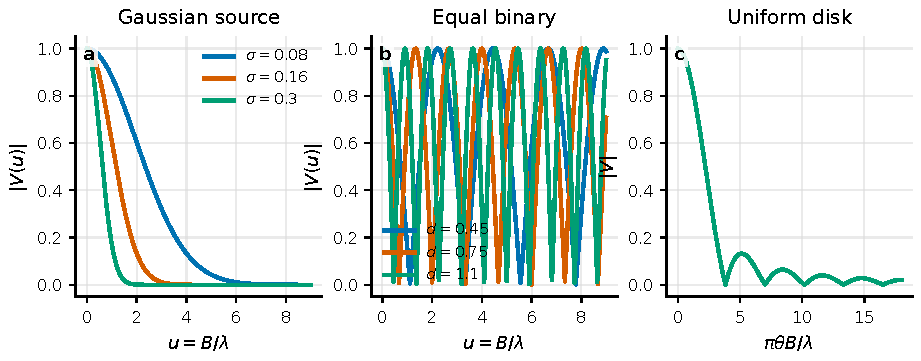
\includegraphics[width=0.9\linewidth]{figures/generated/chapter_01/ch01_fourier_visibility.pdf}
\caption{几种天空亮度结构给出的归一化可见度 \(|V|\) 随空间频率的变化：高斯源平滑下降，等亮双星产生余弦振荡，均匀圆盘因边缘锐利而出现零点和旁瓣。这与本章时间版的"谱线形状 \(\leftrightarrow\) 条纹衰减"完全同构——矩形谱的 sinc 旁瓣，对应均匀圆盘的 Bessel 旁瓣；只是把"频率谱"换成了"天空亮度分布"，"时间延迟"换成了"空间基线"。}
\label{fig:e09-fourier-visibility}
\end{figure}

这一步换轴，威力惊人。维纳--辛钦定理说"\(g^{(1)}(\tau)\) 是功率谱 \(S(\nu)\) 的傅里叶变换"；它的空间孪生兄弟——下一章的主角 van Cittert--Zernike 定理——将说"\(\gamma_{12}\) 是天空亮度分布 \(I(l,m)\) 的傅里叶变换"。于是本章每一条结论都有一个空间对应：条纹衰减的形状告诉我们谱线形状，正如可见度随基线的形状告诉我们\emph{源的角结构}；矩形谱的 sinc 旁瓣，对应均匀圆盘的 Bessel 旁瓣（图 \ref{fig:e09-fourier-visibility}）；相干长度 \(\ell_c\) 之于延迟，正如某个临界基线之于角尺度。把这套时间相干的直觉整体平移到空间，就是我们迈进空间相干与成像的门票。

带着一句话过渡到下一章：\textbf{可见度是一阶相干的读数，而一阶相干沿时间轴给出谱线、沿空间基线给出图像}。第 \ref{chap:e10} 章就从 \(\gamma_{12}\) 出发，用 van Cittert--Zernike 定理把它变成天空的傅里叶分量，再用强度干涉把 \(|\gamma_{12}|^2\) 测出来，一步步走向恒星角直径和成像。

\section{本章要点}
\label{sec:e09-summary}

\begin{itemize}
  \item \textbf{条纹公式。}两路光程差 \(\Delta\) 引入载波相位 \(\delta=2\pi\Delta/\lambda\) 与时间延迟 \(\tau=\Delta/c\)，探测强度 \(I(\delta)=I_1+I_2+2\sqrt{I_1I_2}\,|g^{(1)}(\tau)|\cos(\delta-\varphi(\tau))\)，其中 \(\varphi(\tau)\) 是去掉载波后的缓慢残余相位（谱线对称时为零）。余弦项的振幅正比于一阶相干度 \(|g^{(1)}|\)。
  \item \textbf{可见度就是相干度的读数。}\(\mathcal V=(I_{\max}-I_{\min})/(I_{\max}+I_{\min})=\dfrac{2\sqrt{I_1I_2}}{I_1+I_2}|g^{(1)}(\tau)|\)；等光强时 \(\mathcal V=|g^{(1)}(\tau)|\)。抽象的"电场还记得相位"变成了肉眼可读的条纹对比度。
  \item \textbf{相干长度。}条纹随光程差增大而变淡，特征尺度是 \(\ell_c=c\tau_c\simeq\lambda^2/\Delta\lambda\)：白光约 1\,\(\mu\)m，1\,nm 窄带约 0.3\,mm，MHz 激光约 300\,m。
  \item \textbf{维纳--辛钦桥。}\(g^{(1)}(\tau)\) 是归一化功率谱的傅里叶变换；矩形谱给 \(|g^{(1)}|=|{\rm sinc}(\Delta\nu\tau)|\)（有零点、有旁瓣），洛伦兹谱给 \(|g^{(1)}|=e^{-|\tau|/\tau_c}\)（纯指数）。因此测条纹随延迟的衰减能反推谱线形状——傅里叶变换光谱学的原理。
  \item \textbf{两条路线。}振幅干涉直接测复可见度（含相位）但要求光程稳到波长零头、对大气 piston 敏感；强度干涉只测 \(|\mathcal V|^2\)、丢相位，但只需电子对齐到响应时间零头（见对照表，引出第 \ref{chap:e10} 章）。
  \item \textbf{换轴到空间。}把时间延迟版的 \(g^{(1)}(\tau)\) 换成两点空间版的 \(\gamma_{12}\)，可见度 \(\mathcal V=|\gamma_{12}|\)；它是下一章 van Cittert--Zernike 定理与强度干涉的主角。
\end{itemize}

\medskip
\noindent\textbf{想一想。}
\begin{enumerate}
  \item 一台迈克尔逊干涉仪在白光下只有两臂几乎等长时才见到彩色条纹；换成 \(\Delta\lambda=1\,{\rm nm}\) 的窄带滤光片后，允许的两臂光程差扩大到多少？用式 \eqref{eq:e09-coherence-length} 估一估。
  \item 两路光强比为 \(I_1:I_2=4:1\)，即使光完全相干（\(|g^{(1)}|=1\)），条纹可见度最高能到多少？这说明"看不到满幅条纹"未必意味着不相干。
  \item 若测得可见度随延迟做纯指数衰减 \(\mathcal V(\tau)=e^{-|\tau|/\tau_c}\)，\(\tau_c=1\,{\rm ns}\)，对应的谱线是什么形状、线宽 \(\Delta\nu\) 是多少？换算成波长这条线有多"窄"？
\end{enumerate}
